\documentclass[12pt, a4paper]{article}
%=========================== PACKAGES =============================%

\usepackage[utf8]{inputenc}
\DeclareUnicodeCharacter{00A0}{ }

\usepackage[hmargin=1.5cm,vmargin=1.5cm]{geometry}
\usepackage[brazil]{babel}

\usepackage{longtable}

\usepackage{graphicx}
\usepackage{placeins}
\usepackage{subcaption}
\usepackage{float}

\usepackage{hhline}
\usepackage{courier}

\usepackage{amsmath}
\usepackage{bm}
\usepackage{amsfonts}

\usepackage[hyphens]{url}

\usepackage{listings}
\renewcommand\lstlistingname{Programa}


\usepackage{color} %red, green, blue, yellow, cyan, magenta, black, white
\lstset{language=bash,%
basicstyle=\footnotesize\ttfamily,
breaklines=true,%
keywordstyle=[4]{\color{black}},
frame= single,
}

\lstdefinestyle{nonumbers}
{numbers=none}

\usepackage{multirow}

\usepackage{float}

\usepackage{enumerate}

\begin{document}

%    \maketitle
{\large
\centerline{\textbf{Relatório Exercício Prático 7}}
\centerline{Gustavo Ciotto Pinton 117136}
\centerline{EA979 - Processamento de Imagens}
}

\section* {Explicação}

\begin {enumerate}
  \item A função \texttt{glViewport()} mapeia as coordenadas da cena, em três
  dimensões, para as coordenadas da tela, que apresentam, por sua vez, apenas
  duas dimensões. Tal função recebe quatro parâmetros, sendo eles \textit{x} e
  \textit{y}, que especificam as coordenadas do canto inferior esquerdo, a
  largura \textit{w} e a altura \textit{h} da janela. A modificação dos dois
  primeiros produz um efeito de translação na imagem, sendo que valores
  positivos de \textit{x} \textit{transladam} os objetos para a direita e, de
  \textit{y}, para cima. A imagem \ref{img:xy} é o efeito da execução do
  programa para \textit{x} = 50 e \textit{y} = 50. Nota-se, de fato, o efeito de
  translação. Abaixo, está representada a função com os respectivos parâmetros:
  
  
  \begin{lstlisting}[keywordstyle=\ttfamily, style=nonumbers]
void reshape (int w, int h) {
glViewport (50, 50, (GLsizei) w, (GLsizei) h);
\end{lstlisting}

A mudança do parâmetro \textit{w} para um valor inferior que a largura efetiva
da janela (\textit{w} = 0.5 * \textit{w}, imagem \ref{img:w}) produz, por sua
vez, o efeito de encolhimento (ou escala) nos elementos no eixo \textit{x},
uma vez que a biblioteca \textit{OpenGL} considera apenas aquele intervalo
reduzido na renderização.
Temos, abaixo, a chamada da função responsável por gerar a respectiva imagem.

\begin{lstlisting}[keywordstyle=\ttfamily, style=nonumbers] void reshape (int w, int h) {
void reshape (int w, int h) {
glViewport (0, 0, (GLsizei) w * 0.5, (GLsizei) h);
\end{lstlisting}

Enfim, a imagem \ref{img:xyw} combina as duas manipulações anteriores de forma
a centralizar a cena na área da janela.

\FloatBarrier

\begin{figure}[h!]

\centering

\begin{subfigure}{.33\textwidth}
\centering
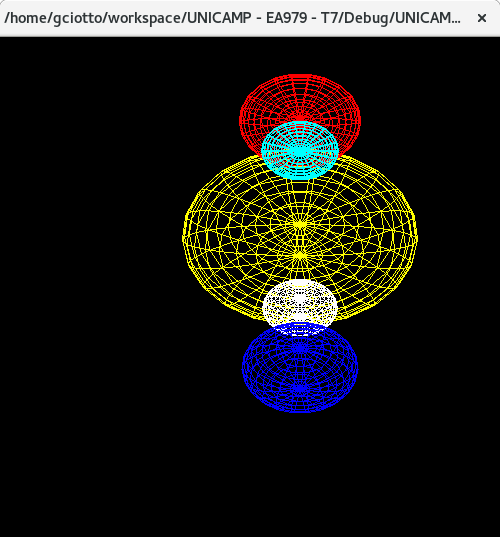
\includegraphics[scale=0.33]{viewportXY}
\caption{\centering Modificação de \textit{x} e \textit{y}.}
\label{img:xy}
\end{subfigure}%
\begin{subfigure}{.33\textwidth}
\centering
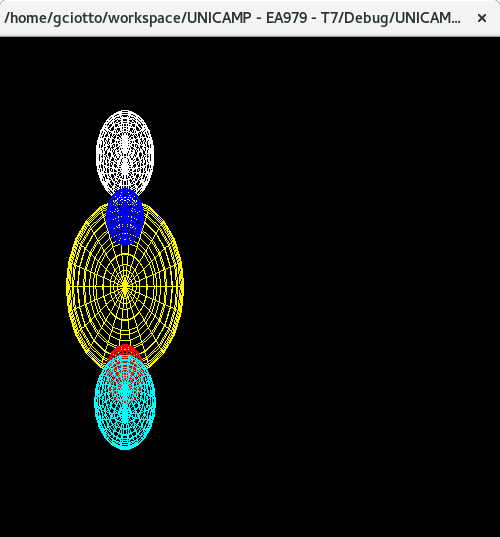
\includegraphics[scale=0.33]{viewportW}
\caption{\centering Modificação de \textit{w}.}
\label{img:w}
\end{subfigure}
\begin{subfigure}{.33\textwidth}
\centering
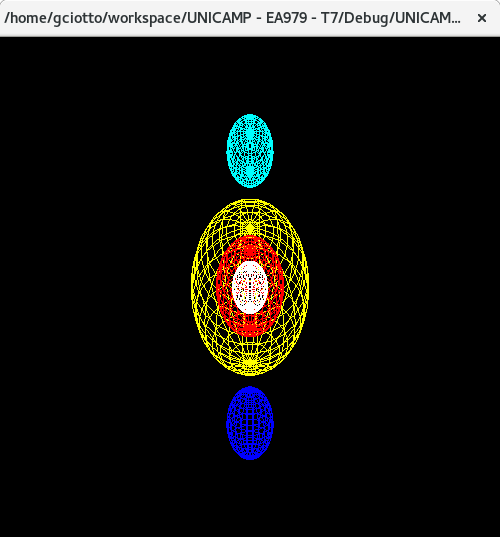
\includegraphics[scale=0.33]{viewportxyw}
\caption{\centering Modificação de \textit{x}, \textit{y} e \textit{w}.}
\label{img:xyw}
\end{subfigure}


\caption{Modificação dos parâmetros da função \texttt{glViewPort()}.}
\end{figure}

\FloatBarrier

A função \texttt{gluPerspective} imita o funcionamento olho humano e é
responsável por adicionar efeitos de profundidade. A modificação das posições
de \texttt{zNear} e \texttt{zFar} não modificam o tamanho com que os objetos são
desenhados, uma vez que especificam os limiares dos dois planos. Por outro
lado, os parâmetros \textit{fovy} e \textit{scale} produzem resultados
diferentes. O primeiro é o ângulo de visão e o segundo, o fator de
proporcionalidade que determina o campo de visão na direção \textit{x}. A
modificação do primeiro para um ângulo superior aumenta o campo de visão e
produz o efeito de \textit{distanciamento} da cena, conforme figura
\ref{img:fovy90}, em que tal parâmetro vale \(90º\). A mudança do segundo gera
alterações semelhantes àquelas produzidas por \texttt{glViewPort()}.

\FloatBarrier

\begin{figure}[h!]

\centering

\begin{subfigure}{.33\textwidth}
\centering
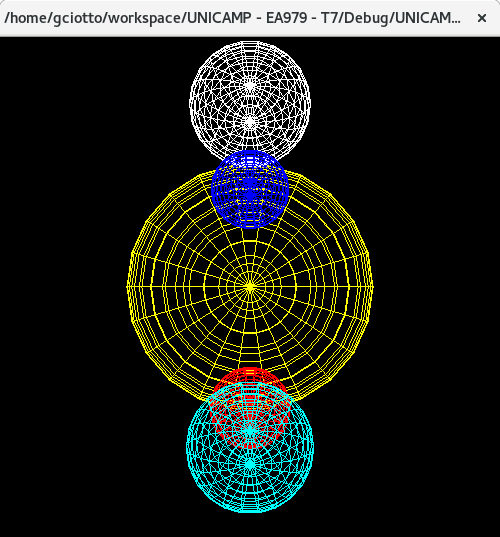
\includegraphics[scale=0.33]{fovy45}
\caption{\centering \textit{fovy} = \(45º\).}
\label{img:fovy45}
\end{subfigure}%
\begin{subfigure}{.33\textwidth}
\centering
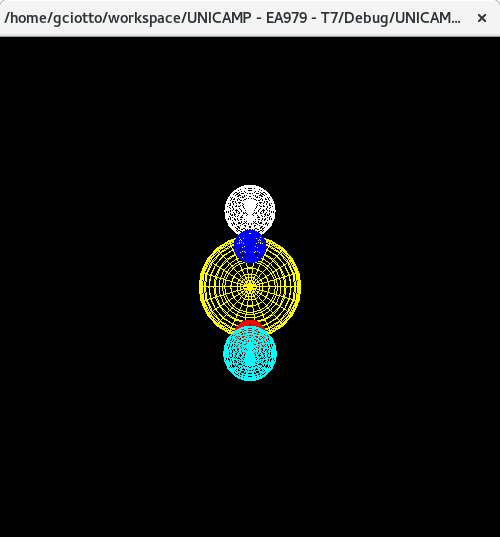
\includegraphics[scale=0.33]{fovy90}
\caption{\centering \textit{fovy} = \(90º\).}
\label{img:fovy90}
\end{subfigure}

\caption{Modificação do parâmetro \textit{fovy} da função
\texttt{gluPerspective()}.}
\end{figure}

\FloatBarrier

\item A fim de desenharmos uma pirâmide, escrevemos uma função chamada
\path{draw_pyramid()}, que chama, por sua, a função \path{glDrawElements()} com
o parâmetro \path{GL_TRIANGLES}. Cada pirâmide pode ser desenhada com 6
triângulos: 2 para a base quadrada e 4 para os lados. 

\vspace{12pt}

Dentro da função \texttt{display()}, realizamos 3 chamadas de
\path{draw_pyramid()}, modificando, em cada caso, a escala e a translação do
sistema de coordenadas através das funções \path{glScalef} e
\path{glTranslatef}. A maior pirâmide possui um \textit{z} mais negativo e, a
menor, um menos negativo. O resultado da execução pode ser conferido na figura
\ref{img:oclusao}. Nota-se que a biblioteca \textit{OpenGL} gerencia os casos de
oclusão gerados pela construção explicada acima, conforme esperado.

\FloatBarrier

\begin{figure}[h!]
\centering
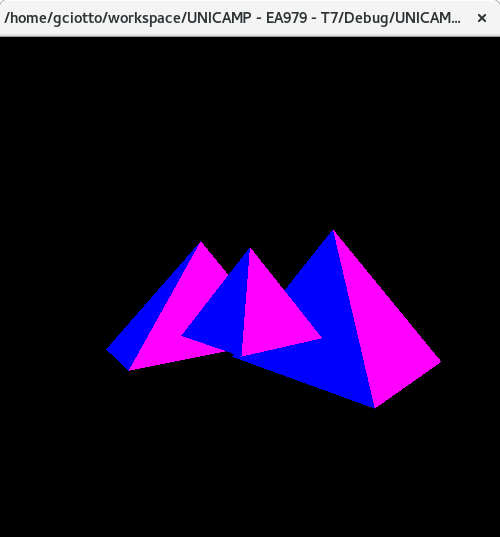
\includegraphics[scale=0.4]{oclusao}
\caption{Renderização de 3 pirâmides.}
\label{img:oclusao}
\end{figure}

\FloatBarrier

\end{enumerate}

\section* {Referências}

\begin {enumerate}
  \item \texttt{glViewport} \textit{reference page}, disponível em
  \url{https://www.opengl.org/sdk/docs/man/html/glViewport.xhtml}.
  \item \texttt{gluPerspective} \textit{reference page}, disponível em
  \url{https://www.opengl.org/sdk/docs/man2/xhtml/gluPerspective.xml}.
\end{enumerate}

\end{document}